\chapter{Background}
	The algorithms and data structures used in this thesis have been introduced and discussed below.

	\section{Levenshtein Distance}
	\label{sec:levenshtein_distance}
		Levenshtein distance \cite{levenshtein1966binary} or evolutionary distance is a concept from information retrieval. It is one of the most common variants of \emph{edit distance} named after the Soviet Russian computer scientist Vladimir Levenshtein. Edit distance \cite {wagner1974string} describes the number of edits that has to be made in order to convert one string to another by performing minimum number of operations like insertions, deletions and substitutions. It is the most common measure to expose the dissimilarity between two strings; the greater the distance, the more different the strings are.
		
		This measure allows to assess similarity between strings (or words) and has many applications that include spell-checking, examining correctness of pronunciation and affinities between dialects, analyzing the DNA structure or web mining. The Levenshtein distance can also be computed between two longer strings.
		
		For example, the Levenshtein distance between ``contest" and ``context" is 1, since just one edit is required to convert one into the other, i.e conte{\bf s}t $\rightarrow$ conte{\bf x}t (substitution of s by x ). Similarly, levenshtein distance between ``incubate" and ``incubus" is 3, since three edits are required to convert one into another and there is no way to do it with fewer than three edits:
		
		\begin{enumerate}
			\item incubat{\bf e} $\rightarrow$ incubat (deletion of ‘e’)
			\item incuba{\bf t} $\rightarrow$ incuba{\bf s} (substitution of ‘t’ by ‘s’)
			\item incub{\bf a}s $\rightarrow$ incub{\bf u}s (substitution of ‘a’ by ‘u’)
		\end{enumerate}
		
		\subsection{Definition}
			Mathematically, the Levenshtein distance between two strings \(a\) and \(b\) is given by \(lev_{a,b}(|a|,|b|)\), where
			\[ lev_{a,b}(i,j) = \left\{ 
				\begin{array}{l l}
					max(i,j) & \quad \text{if \(min(i,j) = 0\),}\\
					min \left\{
					\begin{array}{l}
						lev_{a,b}(i-1,j) + 1\\
						lev_{a,b}(i,j-1) + 1\\
						lev_{a,b}(i-1,j-1) + 1_{(a_i \neq b_j)}
					\end{array} \right.& \quad \text{otherwise.}
				\end{array} \right.\]
			where \(1_{(a_i \neq b_j)}\) is the indicator function equal to \(0\) when \(a_i = b_j\) and \(1\) otherwise.
		
		\subsection{How it works}
			Firstly, with the help of most common approach called dynamic programming, Levenshtein algorithm calculates the minimum number of operations that are required to convert one string to another. A matrix is initialized measuring in the (m,n)-cell the Levenshtein distance between the m-character prefix of one with the n-prefix of the other word. The matrix can be filled from the upper left to the lower right corner. Each horizontal jump corresponds to an insert and each vertical jump corresponds to a deletion. For each of the operation, the cost is normally set to 1. The diagonal jump can have either cost 0 or 1. If the cost is 0, it means that characters match and if it is 1, it means that characters do not match. The cost is always locally minimized by each cell. In this way the number in the lower right corner is the Levenshtein distance between both words. Figure~\ref{levenshtein_matrix} is an example that features the comparison of ``meilenstein" and ``levenshtein" (where `\(= :\)' Match; `\(o :\) Substitution; `\(+ :\) Insertion; `\(- :\)' Deletion).
			
			The two possible paths through the matrix that produces the least cost solution is described in Figure~\ref{levenshtein_path} \footnote{\url{http://levenshtein.net/}}.
			
			\begin{figure}[h!]
				\centering
				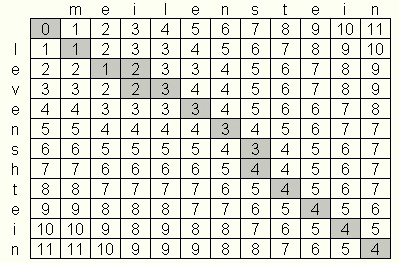
\includegraphics[width=10cm]{levenshtein_meilenstein_matrix.png}
				\caption{Levenshtein distance example for `levenshtein` and `meilenstein` \label{levenshtein_matrix}}
			\end{figure}
			
			\begin{figure}[h!]
				\centering
				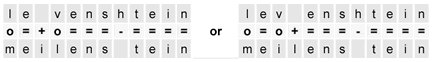
\includegraphics[width=10cm]{levenshtein_meilenstein_path.png}
				\caption{Least cost solution to compute Levenshtein distance  \label{levenshtein_path}}
			\end{figure}

	\section{Hungarian Algorithm}
	\label{sec:hungarian}
		The Hungarian method is an algorithm which finds an optimal assignment for a given cost matrix. It is also known as the \emph{Kuhn-Munkres Algorithm}. The original algorithm \cite{kuhn1955hungarian} had a time-complexity of \(\emph{O}(n^4)\); however, it was later modified to obtain a running time complexity of \(\emph{O}(n^3)\).
		
		\subsection{Definition}
			Assuming that numerical costs are available for each of \(n\) persons on each of \(n\) jobs, the \emph{assignment problem} is the quest for an assignment of persons to jobs so that the sum of the \(n\) costs so obtained is as small as possible.
			
			Let \(c_{i,j}\) be the cost of assigning the \(i^{th}\) resource to the \(j^{th}\) task. We define the cost matrix to be the \(n \times n\) matrix
		\[ C =
			 \begin{bmatrix}
			 	c_{1,1} &	c_{1,2} &	\dots &	c_{1,n} \\
			 	c_{2,1} &	c_{2,2} &	\dots &	c_{2,n} \\
			 	\vdots &	\vdots &	&	\vdots \\
			 	c_{n,1} &	c_{n,2} &	\dots &	c_{n,n}
			\end{bmatrix}
		\]
		
		An assignment is a set of \(n\) entry positions in the cost matrix, no two of which lie in the same row or column. The sum of the \(n\) entries of an assignment is its cost. An assignment with the smallest possible cost is called an \emph{optimal assignment}.
	
	\section{Trie}
	\label{sec:trie}
		Trie \cite{germann2009tightly} is an ordered multi-way tree data structure that is used to store strings over an alphabet. It is a tree data structure that allows string with similar character prefixes to use the same prefix data and store only the tails as separate data. One character of the string is stored at each level of the tree, with the first character of the string stored at the root. Unlike a binary search tree, no node in the tree stores the key associated with that node; instead, its position in the tree shows what key it is associated with. Each node contains an array of pointers, one pointer for each character in the alphabet and all the descendants of a node have a common prefix of the string associated with that node. The root is associated with the empty string and values are normally not associated with every node, only with leaves.
		
		A trie can also be used to represent data types that are objects of any type, for example, strings of integers. Various operations such as searching, deletion, insertion etc. can be performed on a trie. One of the advantages of the trie data structure is that its tree depth depends on the amount of data stored in it. Each element of data is stored at the highest level of the tree that still allows a unique retrieval.
		
		Applications of trie may include sotring a predictive text or an autocomplete dictionary like the one found on a telephone. It is also useful in implementating approximate matcing algorithms including those used in hyphenation and spell checking software.
		
		The insertion to and serching in a \emph{trie} has a time complexity of \emph{O(key\_length)}, each. The space complexity however, is of \emph{O(alphabet\_size * key\_length)}
		
		\begin{figure}[h!]
			\centering
			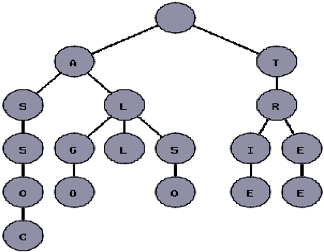
\includegraphics[width=10cm]{trie.png}
			\caption{Trie with the words ``tree", ``trie", ``algo", ``assoc", ``all", and ``also" \label{trie}}
		\end{figure}
	
	\section{Cosine Similarity}	
	\label{sec:cosine_similarity}
		Cosine Similarity \cite{singhal2001modern} measures the similarity between two vectors of an inner product space by measuring the angle cosine between them. A cosine similarity of 1 indicates 0\textdegree, thus having the same orientation, however, a similarity of 0 indicates 90\textdegree. Even though the value of the cosine ranges from \(-1\) to \(1\), the cosine similarity is particularly used in the positive space, i.e., \([0,1]\).
		
		Cosine similarity is commonly used in high-dimensional positive spaces such as in text mining and information retrieval. The popularity of this similarity owes to the fact that it can evaluate very efficiently for sparse vectors as only the non-zero dimensions need to be considered.
		
		\subsection{Definition}
			The cosine of 2 vectors can be obtained by the use of the Euclidean Dot Product:
			\[ a . b = \|a\| \|b\| cos \theta \]
			
			The cosine similarity for 2 vectors \(A\) and \(B\), \(cos \theta \) is representated by
			\[ similarity = cos \theta = \frac{A.B}{\|A\|\|B\|} = \frac{\displaystyle\sum_{i=1}^{n} A_i \times B_i}{\sqrt{\displaystyle\sum_{i=1}^{n} (A_i) ^ 2} \times \sqrt{\displaystyle\sum_{i=1}^{n} (B_i) ^ 2}} \]